\section{Proposed Method}
\label{sec:method}

\subsection{Direct Precision Shrinkage for the EnKF}
\label{sec:dps_enkf}

The Bodnar et al.~\cite{bodnar2016direct} framework was developed for standalone precision matrix estimation and applied to cosmological data by Looijmans et al.~\cite{looijmans2024comparison}. Neither work embedded the estimator inside a sequential filter. We do so here: at each assimilation cycle of the dual EnKF~\eqref{eq:dual_enkf}, we replace the raw sample precision $\hat{\boldsymbol{\Pi}}_S = \mathbf{S}^{-1}$ with the shrinkage estimator
\begin{equation}
\label{eq:direct_precision_method}
\boldsymbol{\Pi}_{\text{LS}} = \alpha^* \hat{\boldsymbol{\Pi}}_S + \beta^* \boldsymbol{\Pi}_0,
\end{equation}
where $\boldsymbol{\Pi}_0$ is a structured target and the coefficients $\alpha^*$, $\beta^*$ are computed from Eqs.~\eqref{eq:alpha_star}--\eqref{eq:beta_star} at every cycle using the current ensemble.

The weight $\alpha^*$ on the sample precision is bounded above by $1 - n/N_e$, reflecting the known positive bias of the Wishart inverse. The remaining weight $\beta^*$ on the target depends on how well $\boldsymbol{\Pi}_0$ aligns with $\hat{\boldsymbol{\Pi}}_S$: when $\text{tr}(\hat{\boldsymbol{\Pi}}_S \boldsymbol{\Pi}_0)$ is large relative to $\|\boldsymbol{\Pi}_0\|_F^2$, more weight goes to the target. Both coefficients are clamped to $[0, 1]$ with $\alpha^* + \beta^* \leq 1$ as a finite-sample safeguard, since the asymptotic guarantees of Bodnar et al.\ do not hold at the ensemble sizes typical of data assimilation ($N_e = 20$--$100$).

Embedding this estimator in the EnKF introduces a consideration absent from standalone estimation: the precision matrix is recomputed at every assimilation cycle, and errors in the analysis state propagate through the forecast model into subsequent cycles. An estimator that is accurate on average but variable from cycle to cycle can accumulate larger errors over a long assimilation window than a slightly biased but stable one. This sequential accumulation effect is not captured by one-shot metrics like Frobenius loss and must be evaluated through filtering experiments (Section~\ref{sec:benchmark}).

\subsection{Shrinkage Targets}
\label{sec:targets}

The four target variants below differ only in their choice of $\boldsymbol{\Pi}_0$. The first three follow Looijmans et al.~\cite{looijmans2024comparison}; the fourth is a domain-agnostic adaptation we propose.

\subsubsection{Identity Target.}

The simplest choice: $\boldsymbol{\Pi}_0 = \mathbf{I}_n$, assuming independent unit-variance priors. This carries no domain-specific information, but the direct precision formulation still produces a valid precision matrix---unlike inverting a shrunk covariance, which can amplify estimation error. Algorithm~\ref{alg:identity} summarises the procedure; the eigenvalue, cosmological, and scaled identity variants (Algorithms~\ref{alg:eigenvalue}, \ref{alg:cosmo}, \ref{alg:scaled}) follow the same template with different choices of $\boldsymbol{\Pi}_0$.

\begin{algorithm}[t]
\caption{Direct Precision Shrinkage (Identity Target)}
\label{alg:identity}
\begin{algorithmic}[1]
\REQUIRE Deviation matrix $\mathbf{DX} \in \mathbb{R}^{n \times N_e}$
\STATE Compute sample covariance: $\mathbf{S} = \frac{1}{N_e-1} \mathbf{DX} \, \mathbf{DX}^T$
\STATE Compute sample precision: $\hat{\boldsymbol{\Pi}}_S = \mathbf{S}^{-1}$
\STATE Set target: $\boldsymbol{\Pi}_0 = \mathbf{I}_n$
\STATE Compute $\alpha^*, \beta^*$ via Eqs.~\eqref{eq:alpha_star}--\eqref{eq:beta_star}
\RETURN $\boldsymbol{\Pi}_{\text{LS}} = \alpha^* \hat{\boldsymbol{\Pi}}_S + \beta^* \boldsymbol{\Pi}_0$
\end{algorithmic}
\end{algorithm}

\subsubsection{Eigenvalue Target.}

A diagonal matrix of the sorted eigenvalues of $\hat{\boldsymbol{\Pi}}_S$: $\boldsymbol{\Pi}_0^{(1)} = \text{diag}(e_1, \ldots, e_n)$ with $e_1 \leq \cdots \leq e_n$. This retains the spectral information of the sample precision while zeroing out off-diagonal correlations, and requires no external domain knowledge. It corresponds to the first precision target ($\boldsymbol{\Pi}_0^{(1)}$) in Looijmans et al.~\cite{looijmans2024comparison}.

\begin{algorithm}[t]
\caption{Direct Precision Shrinkage (Eigenvalue Target)}
\label{alg:eigenvalue}
\begin{algorithmic}[1]
\REQUIRE Deviation matrix $\mathbf{DX} \in \mathbb{R}^{n \times N_e}$
\STATE Compute $\mathbf{S}$, $\hat{\boldsymbol{\Pi}}_S$ as in Algorithm~\ref{alg:identity} (Steps 1--2)
\STATE Compute eigenvalues $e_1 \leq \cdots \leq e_n$ of $\hat{\boldsymbol{\Pi}}_S$
\STATE Set target: $\boldsymbol{\Pi}_0^{(1)} = \text{diag}(e_1, \ldots, e_n)$
\STATE Compute $\alpha^*, \beta^*$ via Eqs.~\eqref{eq:alpha_star}--\eqref{eq:beta_star}
\RETURN $\boldsymbol{\Pi}_{\text{LS}} = \alpha^* \hat{\boldsymbol{\Pi}}_S + \beta^* \boldsymbol{\Pi}_0^{(1)}$
\end{algorithmic}
\end{algorithm}

\subsubsection{Cosmological Target.}

The analytical target from Looijmans et al., derived from the Gaussian power spectrum covariance~\eqref{eq:cosmo_cov}. Each diagonal entry of the target covariance is $T^{(2)}_{ii} = (2/N_{\ell_i}) C_{\ell_i}^2$, encoding cosmic variance at multipole $\ell_i$~\cite{hamilton2006measuring}, and the target precision is its inverse: $\boldsymbol{\Pi}_0^{(2)} = (\mathbf{T}^{(2)})^{-1}$. When the assumed power spectrum model is close to the truth, this provides a stronger shrinkage direction than the generic alternatives.

\begin{algorithm}[t]
\caption{Direct Precision Shrinkage (Cosmological Target)}
\label{alg:cosmo}
\begin{algorithmic}[1]
\REQUIRE Deviation matrix $\mathbf{DX}$, power spectrum $C_\ell$, mode counts $N_\ell$
\STATE Compute $\mathbf{S}$, $\hat{\boldsymbol{\Pi}}_S$ as in Algorithm~\ref{alg:identity} (Steps 1--2)
\FOR{each data element $i$ mapped to multipole $\ell_i$}
    \STATE Compute diagonal covariance target: $T^{(2)}_{ii} = \frac{2}{N_{\ell_i}} C_{\ell_i}^2$
\ENDFOR
\STATE Set target precision: $\boldsymbol{\Pi}_0^{(2)} = (\mathbf{T}^{(2)})^{-1}$
\STATE Compute $\alpha^*, \beta^*$ via Eqs.~\eqref{eq:alpha_star}--\eqref{eq:beta_star}
\RETURN $\boldsymbol{\Pi}_{\text{LS}} = \alpha^* \hat{\boldsymbol{\Pi}}_S + \beta^* \boldsymbol{\Pi}_0^{(2)}$
\end{algorithmic}
\end{algorithm}

\subsubsection{Scaled Identity Target (Novel Adaptation).}
\label{sec:scaled_target}

The cosmological target requires power spectrum data $C_\ell$ and mode counts $N_\ell$ that are unavailable outside cosmology. We propose a domain-agnostic alternative that uses empirical per-variable variances from the sample covariance:
\begin{equation}
\label{eq:scaled_target}
\boldsymbol{\Pi}_0 = \text{diag}\!\left(\frac{1}{2\sigma_1^2}, \ldots, \frac{1}{2\sigma_n^2}\right),
\end{equation}
where $\sigma_i^2$ are the diagonal entries of $\mathbf{S}$. The factor of 2 mirrors the $2/N_\ell$ scaling of the cosmological target in Section~\ref{sec:precision_estimation}. This variant tests how much of the direct precision shrinkage performance depends on domain-specific target knowledge versus the general framework itself. Algorithm~\ref{alg:scaled} summarises the procedure.

\begin{algorithm}[t]
\caption{Direct Precision Shrinkage (Scaled Identity Target)}
\label{alg:scaled}
\begin{algorithmic}[1]
\REQUIRE Deviation matrix $\mathbf{DX} \in \mathbb{R}^{n \times N_e}$
\STATE Compute $\mathbf{S}$, $\hat{\boldsymbol{\Pi}}_S$ as in Algorithm~\ref{alg:identity} (Steps 1--2)
\STATE Read per-variable variances $\sigma_i^2 = \mathbf{S}_{ii}$ for $i = 1, \ldots, n$
\STATE Set target: $\boldsymbol{\Pi}_0 = \mathrm{diag}(1/(2\sigma_1^2), \ldots, 1/(2\sigma_n^2))$
\STATE Compute $\alpha^*, \beta^*$ via Eqs.~\eqref{eq:alpha_star}--\eqref{eq:beta_star}
\RETURN $\boldsymbol{\Pi}_{\text{LS}} = \alpha^* \hat{\boldsymbol{\Pi}}_S + \beta^* \boldsymbol{\Pi}_0$
\end{algorithmic}
\end{algorithm}

Figure~\ref{fig:target_comparison} visualises the four targets at $d = 18$. All are diagonal by construction; they differ only in how the diagonal entries are filled.

\begin{figure}[t]
\centering
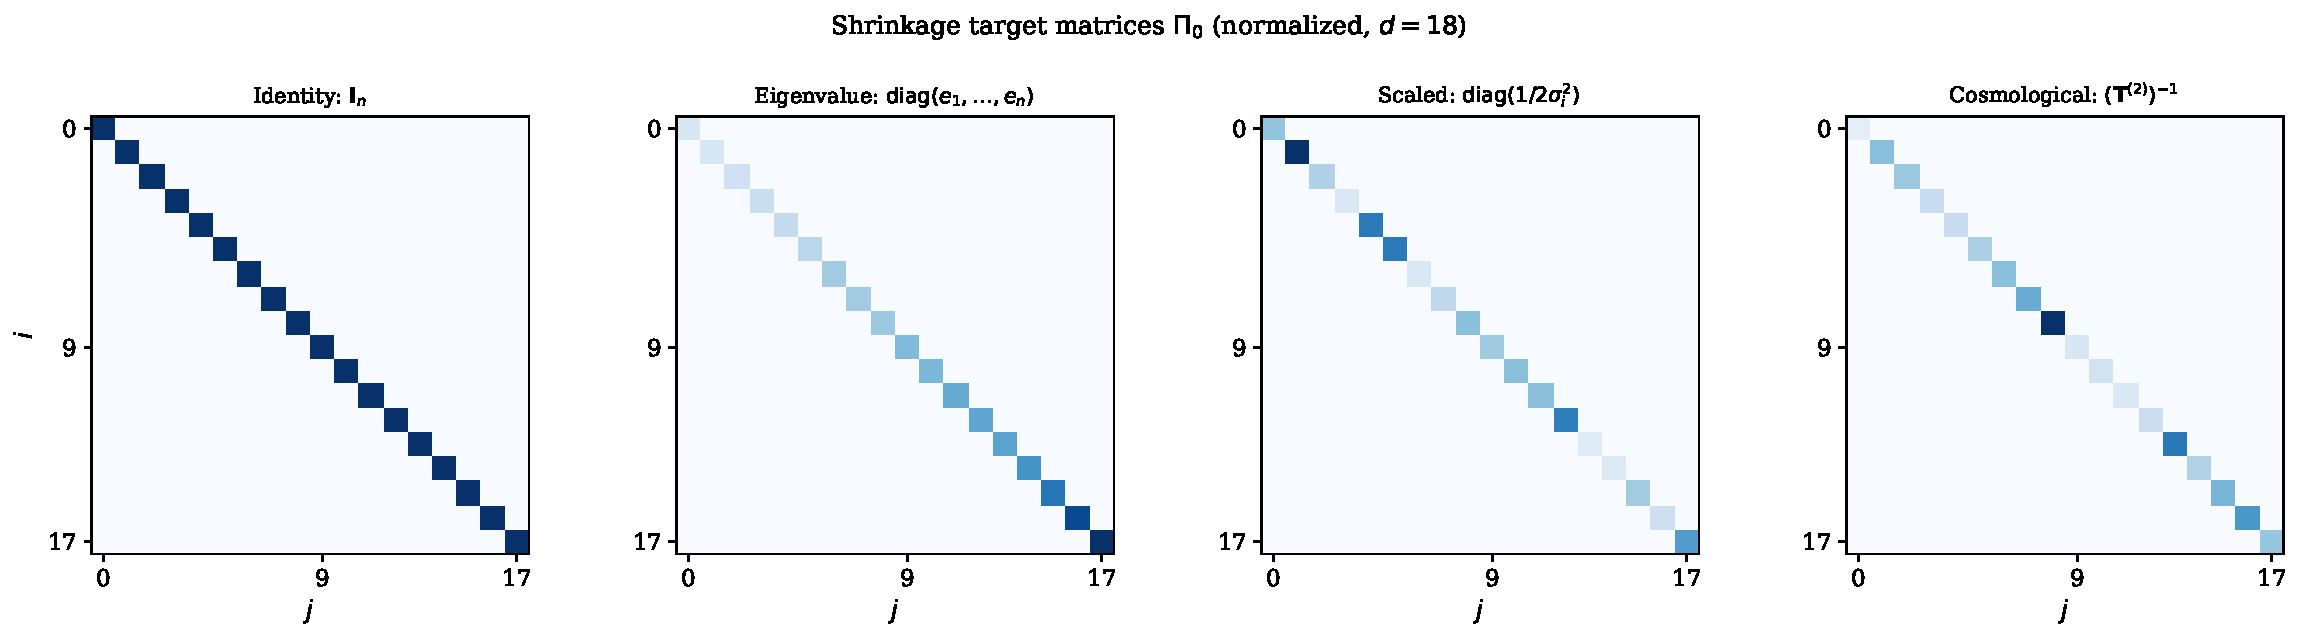
\includegraphics[width=0.85\textwidth]{figures/target_comparison.pdf}
\caption{The four shrinkage target matrices $\boldsymbol{\Pi}_0$ (normalised, $d = 18$). The identity target assigns equal weight to all variables; the eigenvalue target uses the sample precision's spectral information; the scaled and cosmological targets incorporate variance structure from the data or domain knowledge respectively.}
\label{fig:target_comparison}
\end{figure}

\subsection{Computational Complexity}
\label{sec:complexity}

All four direct precision shrinkage variants share a common computational core: forming the sample covariance $\mathbf{S}$ costs $O(n^2 N_e)$, and inverting it to obtain $\hat{\boldsymbol{\Pi}}_S$ costs $O(n^3)$. Computing $\alpha^*$ and $\beta^*$ requires the Frobenius norm $\|\hat{\boldsymbol{\Pi}}_S\|_F^2$, the trace norm $\|\hat{\boldsymbol{\Pi}}_S\|_{\text{tr}}$, and the product $\text{tr}(\hat{\boldsymbol{\Pi}}_S \boldsymbol{\Pi}_0)$, each costing $O(n^2)$ for a dense target or $O(n)$ for a diagonal one. The final linear combination is $O(n^2)$. Since the $O(n^3)$ inversion dominates, all four variants have the same asymptotic cost per assimilation cycle.

They differ in target construction. The identity target requires no computation. The scaled identity reads $n$ diagonal entries of $\mathbf{S}$, costing $O(n)$. The cosmological target similarly costs $O(n)$ given precomputed $C_\ell$ and $N_\ell$ values. The eigenvalue target requires a symmetric eigendecomposition of $\hat{\boldsymbol{\Pi}}_S$, costing $O(n^3)$, which doubles the effective cost of that variant.

Table~\ref{tab:complexity} summarizes the per-cycle cost of each method tested in this work, including the baselines.

\begin{table}[t]
\centering
\caption{Computational complexity per assimilation cycle. $n$: state dimension, $N_e$: ensemble size, $r$: Cholesky bandwidth, $B$: number of NERCOME bootstrap draws.}
\label{tab:complexity}
\begin{tabular}{@{}ll@{}}
\toprule
Method & Cost per cycle \\
\midrule
EnKF (standard)              & $O(n^2 N_e + m^2 N_e)$ \\
EnKF-Cholesky                & $O(n \cdot r \cdot N_e)$ \\
Identity Shrinkage           & $O(n^2 N_e + n^3)$ \\
Scaled Shrinkage             & $O(n^2 N_e + n^3)$ \\
Cosmological Shrinkage       & $O(n^2 N_e + n^3)$ \\
Eigenvalue Shrinkage         & $O(n^2 N_e + 2n^3)$ \\
NERCOME                      & $O(B \cdot (n^2 N_e + n^3))$ \\
Ledoit-Wolf                  & $O(n^2 N_e)$ \\
\bottomrule
\end{tabular}
\end{table}

The modified Cholesky approach avoids the $O(n^3)$ inversion entirely by exploiting banded structure, making it the cheapest option on spatially extended systems where $r \ll n$. Ledoit-Wolf shrinks the covariance directly and does not require inversion ($O(n^2 N_e)$), though the subsequent EnKF solve still involves an $O(m^2 N_e)$ linear system. NERCOME is the most expensive: its $B$ bootstrap resamples (typically $B = 200$) each require a covariance computation and eigendecomposition, resulting in a cost roughly $B$ times that of the other shrinkage methods. On the AR(1) model ($n = 18$, $N_e = 30$), NERCOME takes ${\sim}27$~seconds per 100 cycles versus ${\sim}0.2$~seconds for the other shrinkage methods. On Lorenz~96 ($n = 40$, $N_e = 80$), the gap widens to ${\sim}215$~seconds versus ${\sim}26$~seconds.

All implementations are publicly available in TEDA\footnote{TEDA source code: \url{https://github.com/enino84/TEDA.git}}.
